%%%% Proceedings format for most of ACM conferences (with the exceptions listed below) and all ICPS volumes.
\documentclass[sigconf]{acmart}
%%%% As of March 2017, [siggraph] is no longer used. Please use sigconf (above) for SIGGRAPH conferences.

%%%% Proceedings format for SIGPLAN conferences
% \documentclass[sigplan, anonymous, review]{acmart}

%%%% Proceedings format for SIGCHI conferences
% \documentclass[sigchi, review]{acmart}

%%%% To use the SIGCHI extended abstract template, please visit
% https://www.overleaf.com/read/zzzfqvkmrfzn

%
% defining the \BibTeX command - from Oren Patashnik's original BibTeX documentation.
\def\BibTeX{{\rm B\kern-.05em{\sc i\kern-.025em b}\kern-.08emT\kern-.1667em\lower.7ex\hbox{E}\kern-.125emX}}

% Rights management information.
% This information is sent to you when you complete the rights form.
% These commands have SAMPLE values in them; it is your responsibility as an author to replace
% the commands and values with those provided to you when you complete the rights form.
%
% These commands are for a PROCEEDINGS abstract or paper.
\copyrightyear{2019}
\acmYear{2019}
\setcopyright{acmlicensed}
\acmConference[JCDL, 2019]{JCDL '18: Joint Conference on Digital Libraries}{June 2-6, 2019}{Champaign-Urbana, Illinois}
\acmBooktitle{JCDL '19: Joint Conference on Digital Libraries, June 2-6, 2019, Champaign-Urbana, Illinois}
\acmPrice{}
\acmDOI{}
\acmISBN{}

%
% These commands are for a JOURNAL article.
%\setcopyright{acmcopyright}
%\acmJournal{TOG}
%\acmYear{2018}\acmVolume{37}\acmNumber{4}\acmArticle{111}\acmMonth{8}
%\acmDOI{10.1145/1122445.1122456}

%
% Submission ID.
% Use this when submitting an article to a sponsored event. You'll receive a unique submission ID from the organizers
% of the event, and this ID should be used as the parameter to this command.
%\acmSubmissionID{123-A56-BU3}

%
% The majority of ACM publications use numbered citations and references. If you are preparing content for an event
% sponsored by ACM SIGGRAPH, you must use the "author year" style of citations and references. Uncommenting
% the next command will enable that style.
%\citestyle{acmauthoryear}

%
% end of the preamble, start of the body of the document source.
\begin{document}

%
% The "title" command has an optional parameter, allowing the author to define a "short title" to be used in page headers.
\title{Open Data Publishing by Public Libraries}

%
% The "author" command and its associated commands are used to define the authors and their affiliations.
% Of note is the shared affiliation of the first two authors, and the "authornote" and "authornotemark" commands
% used to denote shared contribution to the research.
\author{Nicholas Weber}
\email{nmweber@uw.edu}
\affiliation{%
  \institution{University of Washington}
  \city{Seattle}
  \state{WA}
}
\author{Bree Norlander}
\orcid{0000-0002-0431-4221}
\email{norlab@uw.edu}
\affiliation{%
  \institution{University of Washington}
  \institution{Technology \& Social Change Group}%Optional
  \city{Seattle}
  \state{WA}
}

%
% By default, the full list of authors will be used in the page headers. Often, this list is too long, and will overlap
% other information printed in the page headers. This command allows the author to define a more concise list
% of authors' names for this purpose.
\renewcommand{\shortauthors}{Weber \& Norlander}

%
% The abstract is a short summary of the work to be presented in the article.
\begin{abstract}
Public libraries in the USA are part of a broad civic information ecosystem that is rapidly adopting transparency legislation aimed at publishing structured open data for public reuse. In this preliminary results paper we look specifically at the open data publishing practices of 85 public libraries in the USA. We find that less than half of these libraries have published any open data, and that there is no relationship between revenue nor staff size and open data publishing practices. Categorizing public library open data by type we find overwhelmingly the most frequent type of open data published by libraries are geospatial (map) information. We use these findings to develop a proposal for public libraries to engage in publishing a core set of open data, and conclude by discussing the potential for reuse of open public library data.
\end{abstract}

%
% The code below is generated by the tool at http://dl.acm.org/ccs.cfm.
% Please copy and paste the code instead of the example below.
%
\begin{CCSXML}
<ccs2012>
<concept>
<concept_id>10002951.10003227.10003392</concept_id>
<concept_desc>Information systems~Digital libraries and archives</concept_desc>
<concept_significance>500</concept_significance>
</concept>
</ccs2012>
\end{CCSXML}
\ccsdesc[500]{Information systems~Digital libraries and archives}
%
% Keywords. The author(s) should pick words that accurately describe the work being
% presented. Separate the keywords with commas.
\keywords{conceptual models, digital libraries}
%All - Please add any keywords or other CCS codes you see fit.

% This command processes the author and affiliation and title information and builds
% the first part of the formatted document.
\maketitle

\section{Introduction}
Over the last decade open government initiatives have spurred the release of valuable public sector information at the federal, state, and municipal levels \cite{chun2010government}. Many of these initiatives include the development of digital library infrastructures, such as repositories or information portals, that enable the publication of and public access to structured data \cite{kitchin2014data}. An initial motivation for adopting open government and open data initiatives is to increase the transparency of government operations, and in turn provide greater political accountability \cite{davies2012promises}. A secondary motivation of open government data programming is the potential for public services to make gains in efficiency through academic and private sector reuse - such as the developers who reuse open data in mobile or web applications that connect citizens to relevant public services offerings \cite{janssen2012benefits, yan2018mining}. Public libraries are beginning to explore service offerings around the use and publication of open data to meet the needs of an increasingly engaged polity  \cite{allen2017strategic}. As most public libraries in the USA are financed through state, county, and city taxes \cite{molz1999civic}, these institutions are also beholden to the same transparency and accountability ordinances around 'open government' as other public service agencies (e.g. Police Departments, Health and Human Services, etc).

In this preliminary results paper we investigate the practices of public libraries as not just services for, but publishers of open government data. We focus in particular on public libraries in 85 USA cities that have either passed open government laws, or established open data infrastructures to publish structured public sector information. Our goals in this research project are to establish a baseline for documenting trends in public libraries publishing open government data. As government funded and provisioned entities we argue that public libraries have rich and valuable public sector information that can contribute to policy making decisions, and can, similar to other public institutions, spur innovation from end-user applications that encourage engagement with unique library resources and service offerings. We hypothesize, however, that as a result of well-documented shortages in technological expertise and data practices more generally \cite{curran2007taking}, public libraries will be immature in their open data publishing efforts. This study will therefore document the publishing practices of USA public libraries at an early stage of broader open government compliance.\\

A second goal of this work is to develop recommendations for what might be a core set of data that all public libraries in the USA can and should publish as open government initiatives mature. We recognize that a number of reporting mechanisms for aggregating data about public libraries already exist. For example, the Institute for Museum and Library Services (IMLS) conducts an annual survey of public libraries to capture general statistics such as library funding levels, circulation trends, program offerings, etc \cite{plsreport2016}. However,  self-reported data from the IMLS annual survey only provides summary statistics, and this type of aggregate data are necessarily limited for meaningful reuse. By describing how USA public libraries can publish full and complete records of their activities to local open data repositories, we argue for the potential to federate public library data into reports that provide more granular information, and in turn compliment existing data sources such as the IMLS's annual statistical reports.

In the following sections we describe the methods used to gather information about the open data publishing practices of 85 public libraries in the USA. We then present preliminary findings from this analysis and answer two broad questions: 1. Are public libraries in the USA publishing open data to city portals?; and if so, 2. What types of open data are public libraries publishing? We conclude with a discussion of the potential for increased open data publishing, and the value that these activities can bring to public library policy development and program planning.

\section{Methods}
To gather a sample of public libraries publishing open data we first randomly selected 85 USA cities from a curated index of 2600 open government data portals from around the world \cite{mercier_we_2015}. For each of the 85 cities listed in the index we recorded the initial url of the data portal, and then tried to verify whether or not the indexed portal link was still valid. If the portal was not still in operation we then attempted to find the city's current open data publishing site. Even though the indexed list of data portals was developed in 2015, we found that 11 of the cities original data portal urls were either incorrect (pointing to an incorrect location), wouldn't resolve, or were forwarded to a different url.

For each city's data portal that was still in operation or that we were able to find via a Google search, we gathered descriptive information about the repository software used to publish the data, the total number of datasets accessible in each portal (we limited Socrata-hosted sites to "type = Datasets"), and searched specifically for data published by or about public libraries. Within each portal we also searched specifically for library-related datasets using queries such as "Library" or "Libr*", and also made use of faceted browsing features such as "categories" or "Data Owner" to locate relevant public library data.

For library related datasets to be considered relevant to our analysis we examined metadata, contents (e.g. variable names), and dataset descriptions. We excluded datasets that contained the keyword "library" but were, in reality, about broader topics such as Boston's "CityScore" dataset which provides "metrics on overall city health based on work done across all facets of the City of Boston" \cite{cityofboston}. Other false positives were removed based on the identified publisher. For example, the City of Seattle has a number of datasets that are published to the portal by users who have performed a specific analysis of that public library's data, but were not officially published by the Seattle Public Library.

In addition to searching data portals for relevant library data we also looked to broader statistical indexes and data census information to understand the open data publishing practices of the cities in our sample. From the Open Knowledge Foundation's (OKFN) 2016 USA City Open Data Census -  a project that inventoried the types and quality of open data published in over 150 USA cities - we recorded each city's overall openness score \footnote{http://us-city.census.okfn.org/year/2016}. An overall openness score is calculated by combining a 100-point evaluation for 19 different types of open data. For example, a city will receive a 100-point score for "open crime data" if the city publishes this information in a machine-readable format, is free to download, etc. Combining the 19 different scores by type , a city can at best score a 1900 in the OKFN census. We hypothesize that cities with high overall openness scores in the census will be more likely to publish public library data, as it speaks to the city's commitment to making public sector information accessible and the maturity of supporting data infrastructures.

We also gathered statistical information about each of the libraries in our sample from the 2016 IMLS Public Library survey \footnote{https://data.imls.gov/Public-Libraries-Survey/Public-Libraries-Survey-2016-Library-Systems-Admin/grpq-tgei}. Several cities in our initial dataset had multiple entries in the IMLS survey (e.g. Austin which has four different library systems within the city limits: Austin Public, Lake Travis Community, Westbank Community, and Wells Branch Community). For this preliminary study, rather than investigate each occurrence and disaggregate the statistical information, we simply removed cities with multiple entries from our sample. We also removed cities with insufficient data or broken links to data (Reno, Lubbock, Jacksonville), cities with custom portals that made it difficult to search for and/or total datasets, and Minneapolis which has no corresponding library in the IMLS data due to a county-wide library system. This resulted in a final dataset that included 62 cities, including information we gathered from our own inventory as well as supplementary IMLS survey statistics.
\section{Findings \& Discussion}
Below we present findings from our analysis, which are addressed at answering two broad questions: 1. Are public libraries in the USA publishing open data to city portals?; and if so, 2. What types of open data are public libraries publishing?

\subsection{Libraries Publishing Open Data}
All 62 cities that remained in our sample were classified by the IMLS as City (Large, Midsize, or Small) or Suburban (Large) library systems. This designation in the IMLS Public Library survey is based on the geocoded latitude and longitude values of a library's main branch street address. The size subcategory (Large, Midsize, or Small) is based on the National Center for Education Statistics (NCES) locale coding system \cite{plsreport2016}. That all library systems in our sample were either categorized as a City or Suburb system should be interpreted as a result of the adoption of open government initiatives and open data infrastructure development.  Previous research has shown that throughout Europe \cite{conradie2012exploring} and the USA \cite{bearfield2017can} large municipalities, including cities and well funded suburbs \cite{mergel2018open}, are the earliest adopters of the transparency initiatives that result in open data publishing. Our sample, gathered from an indexed list of existing open data portals necessarily reflects this systemic bias in open data publishing practices.

Of the 62 cities that remained in our sample less than half (n = 27) have published any library related data. In figure 1 we show the frequency distribution of all cities in our sample that published more than 1 library related dataset (n=10). The library that published the most datasets (n= 55) was Chicago, a large metropolitan city that represents one of the longest running and most robust open data programs in the USA \cite{kassen2013promising}. That less than half of the cities in our sample have published library related open data, and only ten had published more than one dataset, confirms our hypothesis that public libraries conformance with open government initiatives is immature.

After confirming the frequency of public library open data publishing we attempted to better understand how these practices related to the overall open data publishing of a particular city. For example, we would expect that Chicago, with a long-standing open data program, might simply be publishing more library related data as a spillover over effect of  the existing human and technical infrastructure that is available to support a library's publishing efforts. We also suspected that cities with high overall 2016 USA City Open Data Census Scores would be more likely to publish public library data. From the IMLS annual survey data there are a number of potentially relevant variables that can shed light on what influences the practices of public libraries as open data publishers - namely,  the total revenue of a city's public library system (as a proxy to available funding), and the number of full time staff (as a proxy to labor size). One would expect that with a larger annual revenue or a larger staff a public library could invest more time and effort into complying with transparency initiatives, and overall managing data for public release.

To investigate these hypotheses, we ran a simple linear regression with the "count of library datasets" as the dependent variable against the the independent variables (each in turn), "total annual revenue," "total staff," and "Open Data Census Score." We found no significant relationship between library datasets and revenue (though "total overall datasets available in a city" does have a statistically significantly positive correlation to library revenue with a p-value of $2.35e^{-12}$). Regression analysis of "count of library datasets" and  "total staff" produced a nearly statistically significant correlation with a p-value of 0.08. While this value does not demonstrate a strong enough correlation to reject the null hypothesis (that there is no relationship between the variables "staff size" and "total library datasets published") we do believe that the IMLS statistical data may be relevant for future exploration. Finally, simple linear regression showed no statistically significant relationship between library datasets and their corresponding open data census scores. While the largest provider of public data, Chicago, does appear as our 5th highest census score city, the second largest provider, Durham, does not even make the top ten in census scores.

In summary, given the small sample size of libraries in this analysis we find no significant correlation between either staff size, nor the total annual revenue of a public library as indicating a propensity to engage open data publishing. Staff and revenue are likely confounding variables (in fact they are highly correlated with a Pearson correlation coefficient of 0.95). However, that they have no correlation with publishing practices further emphasizes the fact that public libraries are part of, and embedded in, a broader civic information ecosystem that often evolves piecemeal through slow and steady maturation \cite{attard2015systematic}.

\subsection{Types of Public Library Open Data}
To better understand and describe the types of open data that were being published by public libraries we further analyzed the contents and formats of each dataset in our sample (n=27 libraries that had actually published 1 or more open datasets). We began by listing the title of all datasets, and where possible the portal (repository) categories that these data were published under. From these general open data categories, we created a categorization to describe the type of library data that were being published. This categorizations included the following 10 types of structured public library data: Geospatial, Facilities, Catalog \& Circulation, Patrons, Public Records, Events \& Calendar, Human Resources, Financial, Utilities, Technology Offerings (for a complete definition of each category please see the full dataset).

Applying this categorization to the 27 public libraries that published open data we find that the most frequent type of data published are Geospatial (n= 27) followed by Catalog \& Circulation (n=7) and information about Patrons (n=7) (see Figure 2). In almost every instance of Geospatial data published by a library there was an accompanying shapefile.  It is not surprising that geospatial data appears to be the most frequent category of data published by libraries in our sample; In fact, geospatial information is one of the most popular, by format, of all open government data published in the USA \cite{washington2016open}.

Catalog \& Circulation data are published second most frequently in our sample, but it is still somewhat surprising that this type of data is not more frequently a part of the publishing practice of a library engaged in open data programs. Circulation data in particular are already well structured and often described as the most valuable asset for data-driven collection development and evaluation \cite{knievel2006use}. We hypothesize that libraries not publishing this data is due to a lack of skills in anonymizing what might be patron records containing personally identifiable information (PII) - which is a recognized hurdle and future challenge for releasing and making use of circulation data \cite{renaud2015mining}. .

Overall, facilities information, patron data (e.g. de-identified circulation records by branch), and technology offerings (e.g. number of laptops available for lending, computer terminals, etc.) were rarely published by the libraries in our sample. We expect that this type of data is readily available to library staff in structured (or structurable) formats, and therefore represent candidate data types for public libraries to easily and efficiently publish as their first open data contribution to a city portal. We further discuss this potential in the following section.

\begin{figure}
\centering
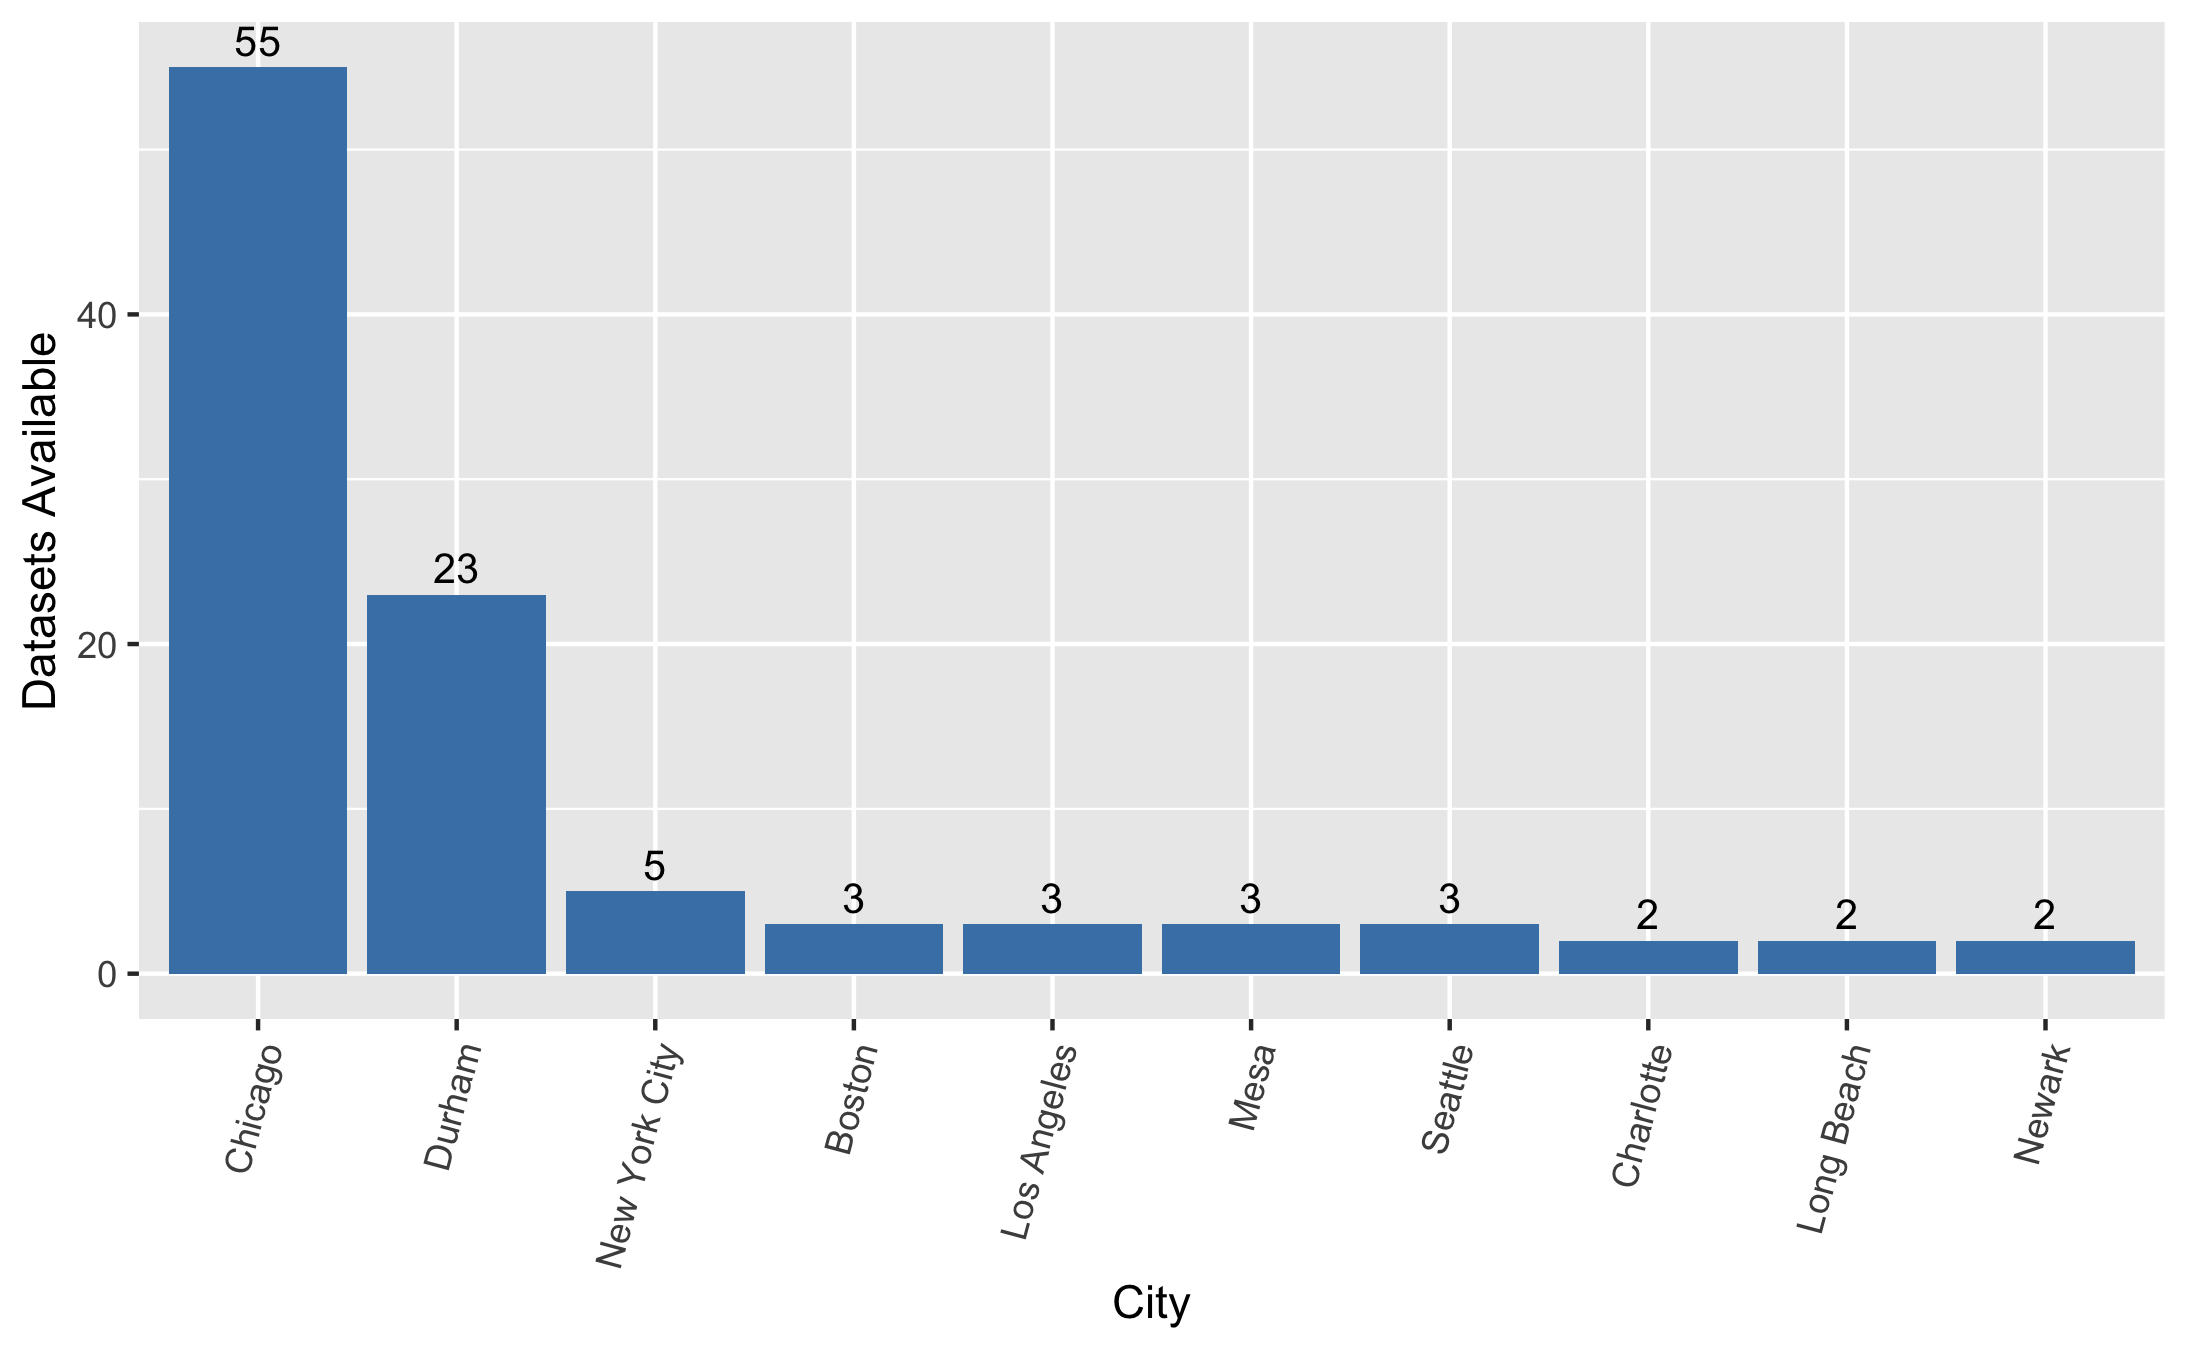
\includegraphics[width=0.45\textwidth]{images/cities_barchart_sorted_morethanone.png}
\caption{\label{fig:categories}Frequency distribution of all cities the sample that published more
than 1 library-related dataset.}
\end{figure}

\begin{figure}
\centering
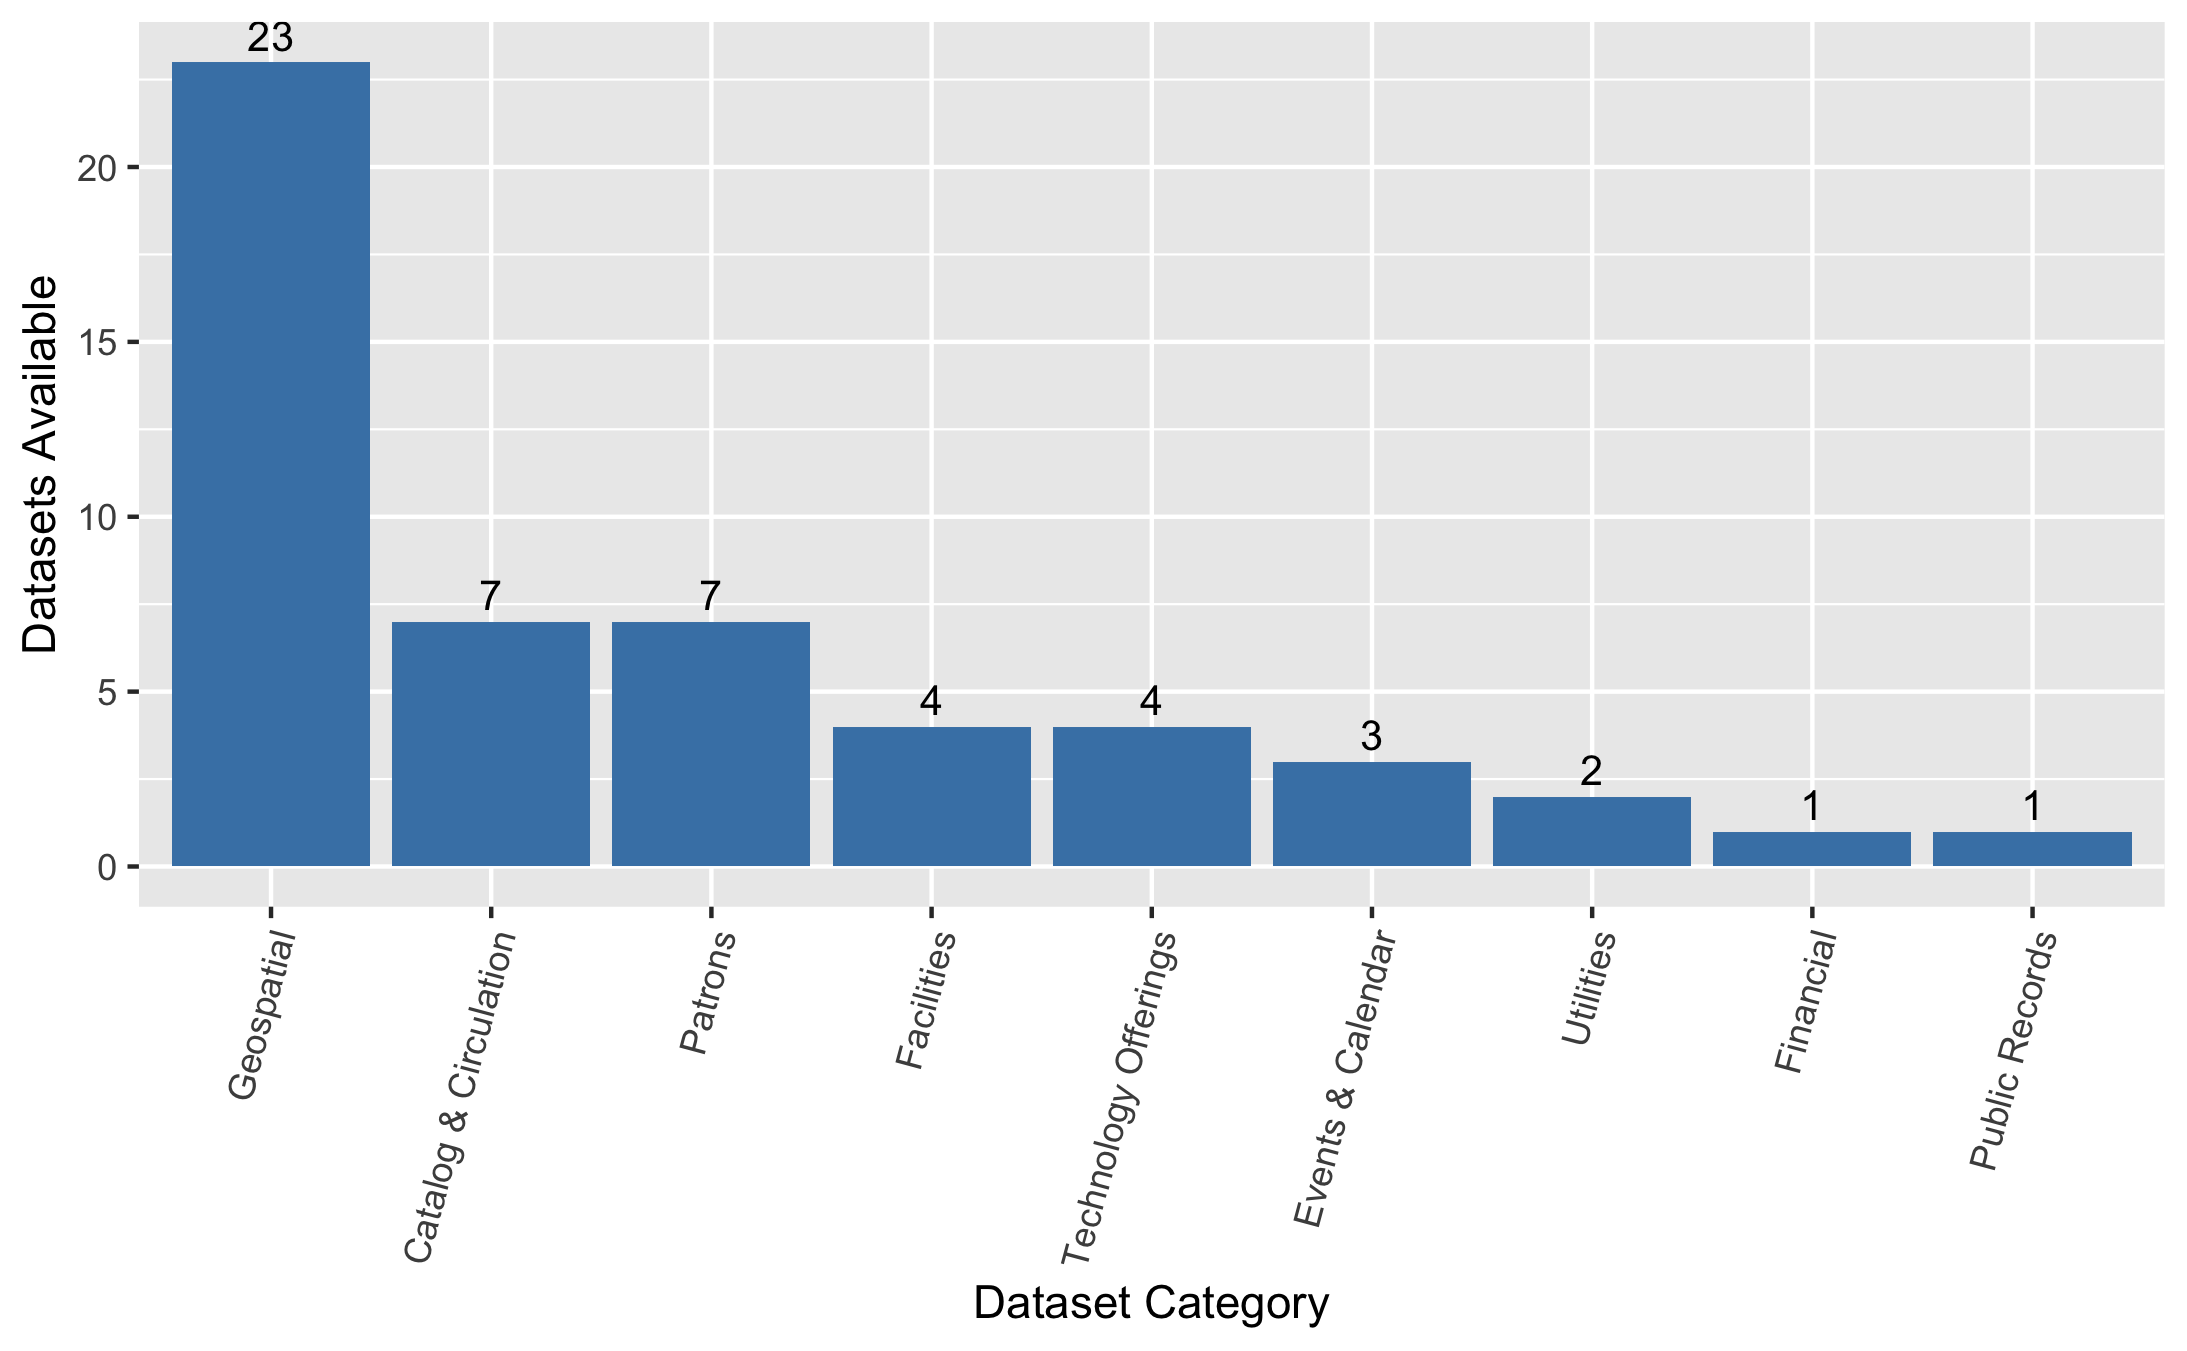
\includegraphics[width=0.45\textwidth]{images/categories_barchart_sorted.png}
\caption{\label{fig:categories}Total library datasets in each category.}
\end{figure}

\section{Conclusion \& Future Work}
Through an empirical study of the open data publishing practices of 85 cities in the USA we have demonstrated that: 1. Less than half of the libraries in our sample are actively publishing open data (n=27), and a much smaller number are publishing more than one dataset (n=10); 2. We found no relationship between the size of a library's annual revenue and their propensity to publish open data, but did find a weak correlation between staff size and propensity to publish open data; 3. By examining specific types of published open library data we find that most datasets contain geospatial information. These findings demonstrate that open data publishing by public libraries is relatively immature compared to other city entities (e.g. Fire departments, health and human services, etc). However, we believe that public libraries are also well positioned to make their data more accessible due to the fact that circulation, patron, technology offerings, and event data are already broadly collected and likely well structured.

In future work we believe there is a need to better understand not just the open data publishing practices, but also the data collection efforts of local public libraries. Future steps might include working with libraries to inventory their current holdings, and understand what types of data might be most useful in alignment with local and national measurement systems for evaluation of public services \cite{smith2017landscape}. We also see a great potential to use the type categories of library open data developed in this paper to suggest structured data that can easily be published by public libraries. Further, there is the potential to share best practices in publishing certain types of open public library data, and develop professional development and outreach materials to help public library staff understand challenges in releasing this type of public sector information.

Finally, there may be questions as to the utility of public libraries investing scarce resources in publishing open data. We return to the second motivation of open government initiatives described in the Introduction section - there are many unanticipated reuses of structured open data that can spur public and private sector innovation, and lead to gains in public engagement. As evidence, we point to the platform Kaggle where datasets are published, curated, and analyzed by a large social network of data scientists. On Kaggle one can currently find analysis and conversations around public library data made available by San Francisco, Seattle, Oakland, New York City, and a number of other cities \footnote{e.g. https://www.kaggle.com/bengin/mastering-the-sf-library-data}. This community is building models to understand patron behavior, and identify resource consumption patterns in public library systems. The online collective action that could facilitate insights for libraries and cities is indeed a potential value already being realized, and we believe this wisdom of the crowd insight will only improve with greater public library data accessibility.

\section{Data Availability}
The data described in this paper, further documentation about the methods used, and the images included are openly accessible at:  https://github.com/OpenDataLiteracy/JCDL-2019-
OpenDatainPublicLibraries

%
% The acknowledgments section is defined using the "acks" environment (and NOT an unnumbered section). This ensures
% the proper identification of the section in the article metadata, and the consistent spelling of the heading.
\begin{acks}
This research was supported in part by IMLS grant # RE-40-16-0015-16.
\end{acks}

%
% The next two lines define the bibliography style to be used, and the bibliography file.
\bibliographystyle{ACM-Reference-Format}
\bibliography{sample-base}

%
% If your work has an appendix, this is the place to put it.
%\appendix

\end{document}
